\normaltrue \difficilefalse \tdifficilefalse
\correctionfalse
%\UPSTIidClasse{11} % 11 sup, 12 spé
%\newcommand{\UPSTIidClasse}{11}

\exer{ $\star$ \label{B2:16:69}}
%% CCP MP 2007
\setcounter{numques}{0}
\UPSTIcompetence[2]{B2-16}
\index{Compétence B2-16}

\index{Train d'atterrissage A350}
\index{Hyperstatisme}

\ifcorrection
\else
\textbf{Pas de corrigé pour cet exercice.}
\fi

\ifprof
\else
La configuration du train d’atterrissage de l’avion A350-900 est de type tricycle avec :
\begin{itemize}
\item deux atterrisseurs principaux (gauche et droit) attachés sur la voilure, légèrement à
l’arrière du centre de gravité $G$ de l’avion et de part et d’autre du plan de symétrie
vertical $\left(O, \vect{x}, \vect{z}\right)$ de l'avion. Ils supportent l’essentiel du poids de l’avion ;
\item un atterrisseur auxiliaire situé sous le nez de l’avion, qui assure l’équilibre longitudinal
de l’avion au sol et permet de manoeuvrer.
\end{itemize}
Les atterrisseurs principaux sont équipés de quatre roues chacun, tandis que
l’atterrisseur auxiliaire est équipé de deux roues.
\end{itemize}


\begin{center}
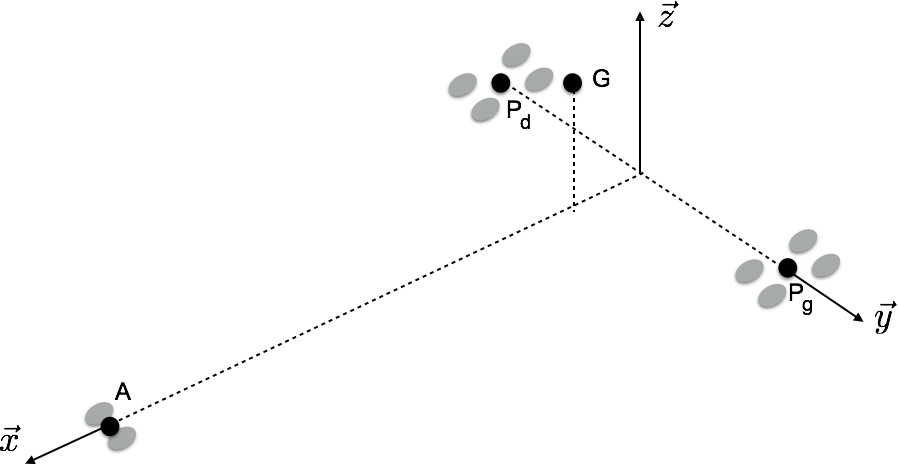
\includegraphics[width=\linewidth]{69_01}
\end{center}

Les mobilités entre les différents éléments de l’avion (roues,
fuselage…) ne sont pas considérées ; ces éléments ne forment donc qu’une seule
classe d’équivalence désignée « avion ».

\fi

\question{Réaliser le graphe des liaisons.}
\ifprof
\else 
\fi

\question{Déterminer le degré d’hyperstatisme d’une modélisation de la liaison avion-sol
dans laquelle chaque contact roue-sol serait considéré ponctuel.}
\ifprof
\else 
\fi

Pour simplifier l’étude, les actions mécaniques de contact entre chaque atterrisseur et
le sol sont modélisées globalement par un effort ponctuel vertical. Ainsi la modélisation
introduit trois liaisons ponctuelles de normales $(A, \vect{z})$ (atterrisseur
auxiliaire), $(P_g, \vect{z})$ (atterrisseur principal gauche) et $(P_d, \vect{z})$ (atterrisseur principal droit).

\question{Démontrer que ce modèle simplifié est isostatique.}
\ifprof
\else 
\fi
 
 

\ifprof
\else

\noindent\footnotesize
 \fbox{\parbox{.9\linewidth}{
 Éléments de corrigé : 
 \begin{enumerate}
\item .
%\item $h=8$.
\item .
 \end{enumerate}}}
\normalsize

\begin{flushright}
\footnotesize{Corrigé  voir \ref{B2:16:69}.}
\end{flushright}%
\fi